\begin{activity} \label{A:10.6.11} 
  Consider the function $f$ defined by $f(x,y) = 2x^2 - xy + 2y$.  
  \ba
\item Find the gradient $\nabla f(1,2)$ and sketch it on Figure
  \ref{F:10.6.activity.empty}. 

  \begin{figure}[ht]
    \begin{center}
      \includegraphics{figures/fig_10_6_activity_empty.eps}
    \end{center}	
    \caption{A plot for the gradient $\nabla f(1,2)$.}
    \label{F:10.6.activity.empty}
  \end{figure}

\item Sketch the unit vector $\vz = \left\langle-\frac1{\sqrt{2}},
    -\frac1{\sqrt{2}}\right\rangle$ on Figure
  \ref{F:10.6.activity.empty} with its tail at $(1,2)$.
  Now find the directional derivative $D_{\vz}f(1,2)$.  

\item What is the slope of the graph of $f$ in the direction $\vz$?  
  What does the sign of the directional derivative tell you?  

\item Consider the vector $\vv = \langle 2,-1\rangle$ and sketch $\vv$
  on Figure \ref{F:10.6.activity.empty} with its tail at $(1,2)$.
  Find a unit vector $\vw$ pointing in the same direction of $\vv$.
  Without computing $D_{\vw}f(1,2)$, what do you know about the sign
  of this directional derivative?  Now verify your observation by
  computing $D_{\vw}f(1,2)$.

\item 
%If $\theta$ is the angle between $\nabla f(1,2)$ and $\vu$, then
%  $$
%  D_{\vu}f(1,2) = \nabla f(1,2)\cdot \vu = |\nabla
 % f(1,2)||\vu|\cos\theta = |\nabla
%  f(1,2)|\cos\theta,
 % $$
 % since $\vu$ is a unit vector.  
 In which direction (that is, for what unit vector $\vu$) is $D_{\vu}f(1,2)$
  the greatest?  What is the slope of the graph in this direction?

\item Corresponding, in which direction is $D_{\vu}f(1,2)$ least?  What is the slope of the graph in this direction?

\item Sketch two unit vectors $\vu$ for which $D_{\vu}f(1,2) = 0$ and
  then find component representations of these vectors.

\item Suppose you are standing at the point $(3,3)$.  In which
  direction should you move to cause $f$ to increase as rapidly as
  possible?  At what rate does $f$ increase in this direction?

  \ea

\end{activity}

\begin{activitySolution}
\ba 
\item The gradient of $f$ at $(1,2)$ is
\[\nabla f(1,2) = \langle f_x(1,2), f_y(1,2) \rangle = \langle 2,1\rangle.\]
A plot of  $\nabla f(1,2)$ is shown below.

\item A plot of $\vz$ is shown below. The directional derivative $D_{\vz}f(1,2)$ is 
\[D_{\vz}f(1,2) = f_x(1,2)\left(-\frac{1}{\sqrt{2}}\right) + f_y(1,2)\left(-\frac{1}{\sqrt{2}}\right) = -\frac{3}{\sqrt{2}}.\]

\item The directional derivative $D_{\vz}f(1,2)$ tells us the slope of $f$ in the direction of $\vz$ at the point $(1,2)$, so this slope is $-\frac{3}{\sqrt{2}}$. The fact that $D_{\vz}f(1,2)$ is negative tells us that the graph of $f$ is decreasing in the direction of $\vz$ from the point $(1,2)$. 

\item The angle between the vector $\vv$ or the vector $\vw = \frac{1}{|\vv|} \vv = \frac{1}{\sqrt{5}}\langle 2, -1 \rangle$ (shown below) and $\nabla f(1,2)$ is acute, so we expect $f$ to be increasing in this direction. Note that 
\[D_{\vw}f(1,2) = \frac{1}{\sqrt{5}}(f_x(1,2)(2) + f_y(1,2)(-1)) = \frac{3}{5}\sqrt{5}.\] 

   \begin{center}
      \resizebox{!}{2.4in}{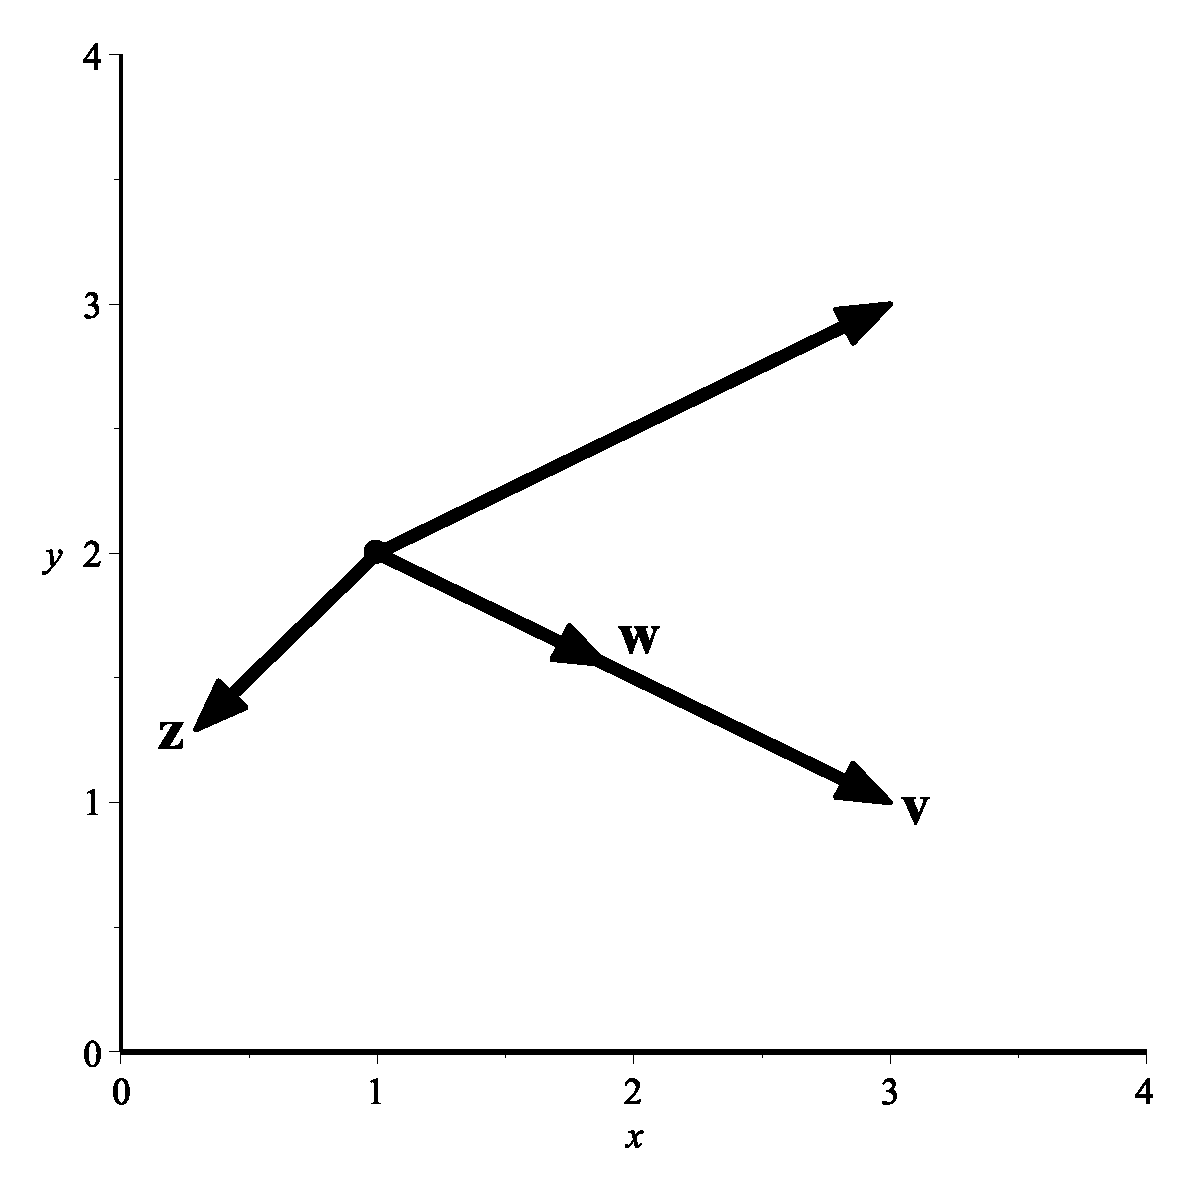
\includegraphics{figures/fig_10_6_Act_11_gradient.eps}}
    \end{center}
    
\item We know that $f$ increases most rapidly in the direction of the gradient. So $D_{\vu}f(1,2)$ is greatest when \[\vu = \frac{1}{|\nabla f(1,2)|} \nabla f(1,2) =  \frac{1}{\sqrt{5}}\langle 2,1 \rangle.\]
The slope of the graph of $f$ in the direction of $\nabla f(1,2)$ at the point $(1,2)$ is
\[D_{\vu}f(1,2) = \frac{1}{|\nabla f(1,2)|}(f_x(1,2)(f_x(1,2)) + f_y(1,2)(f_y(1,2))) = |\nabla f(1,2)| = \sqrt{5}.\]

\item the function $f$ decreases most rapidly in the direction opposite of the gradient. So $D_{\vu}f(1,2)$ is least when 
\[\vu = -\frac{1}{|\nabla f(1,2)|} \nabla f(1,2) =  -\frac{1}{\sqrt{5}}\langle 2,1 \rangle.\]
The slope of the graph of $f$ in the direction of $-\nabla f(1,2)$ at the point $(1,2)$ is
\[D_{\vu}f(1,2) = - |\nabla f(1,2)| = -\sqrt{5}.\] 

\item Recall that $D_{\vu}f(1,2) = \nabla f(1,2) \cdot \vu$, so $D_{\vu}f(1,2) = 0$ when $\vu$ is perpendicular to $\nabla f(1,2)$. By inspection, two such vectors are $\frac{1}{\sqrt{5}}\langle 1, -2 \rangle$ and $\frac{1}{\sqrt{5}}\langle -1,2 \rangle$.  

\item The direction in which $f$ increases most rapidly at the point $(3,3)$ is 
\[\vu=\frac{1}{|\nabla f(3,3)|}\nabla f(3,3) = \frac{1}{\sqrt{82}}\langle 9, -1 \rangle.\]
The rate of increase of $f$ in this direction is 
\[D_{\vu} f (3,3) = |\nabla f(3,3)| = \sqrt{82}.\]
\ea

\end{activitySolution}

\aftera
